\chapter{Level 2: Generate and analyse traffic on your network}

\section{Protocol Analysis}

To generate network traffic, we utilised the \texttt{iperf} tool to create UDP traffic between the machines in our network. We chose UDP traffic because the \texttt{iperf} tool automatically displays performance metrics such as jitter and packet loss when sending UDP traffic. We then analysed the captured traffic using Wireshark, a powerful network protocol analyser, to gain insights into the network's behaviour and performance.

Figure~\ref{fig:WiresharkProtocolAnalysis} provides a comprehensive view of the protocol hierarchy of the captured traffic. We used Wireshark's built-in filters to focus specifically on the UDP traffic generated by the \texttt{iperf} tool. The protocol analysis revealed that the TCP protocol dominated the network communication when including TCP traffic, likely due to the background connections the VM was making to the rest of the KCL network. However, the UDP traffic generated by the \texttt{iperf} tool was visible as a separate protocol in the Wireshark analysis, allowing us to isolate and analyse the UDP traffic independently.

\begin{figure}[H]
\centering
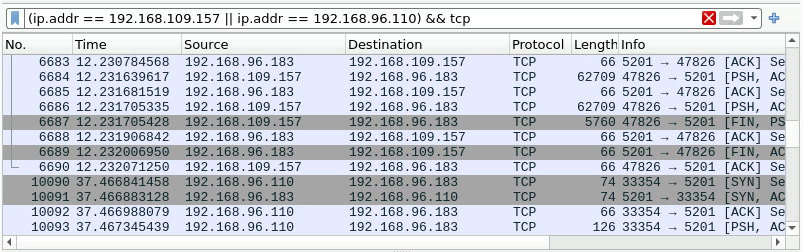
\includegraphics[width=0.8\textwidth]{img/level2/level2-server-protocol-analysis.png}
\caption{Wireshark Protocol Analysis}\label{fig:WiresharkProtocolAnalysis}
\end{figure}

\section{Packet Analysis}

We can examine individual packets at the packet level to understand their structure and contents. Figure~\ref{fig:WiresharkPacketAnalysis} displays a UDP packet captured during the traffic generation. The packet details show the source and destination IP addresses, ports, packet length, and checksum. This information is crucial for troubleshooting and identifying any anomalies in the network communication. While these packets are not malicious in this case, we can use this information to identify malicious packets at future levels.

\begin{figure}[H]
\centering
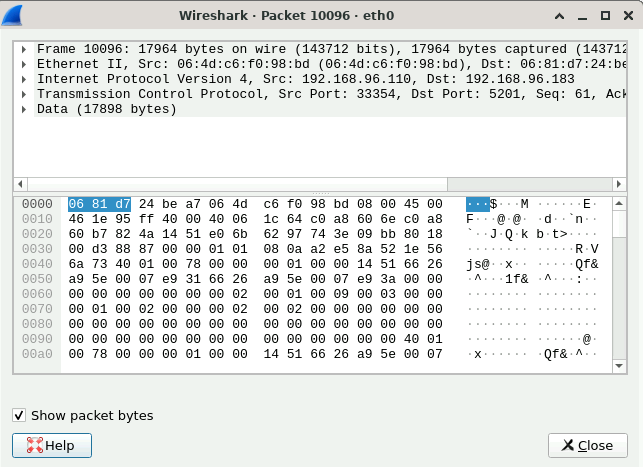
\includegraphics[width=0.8\textwidth]{img/level2/level2-server-packet-analysis.png}
\caption{Wireshark Packet Analysis}\label{fig:WiresharkPacketAnalysis}
\end{figure}

\section{Flow Analysis}

Our analysis extended to the flow level, where we used Wireshark's Conversations feature to group packets into logical connections between endpoints. Figure~\ref{fig:WiresharkFlowAnalysis} presents the UDP conversations in the captured traffic. Each row represents a unique UDP connection, showing the source and destination addresses, the number of packets exchanged, and the total amount of data transferred. This flow-level analysis demonstrates how we used \texttt{iperf} to generate UDP traffic between the machines in our network, setting up the attacker as an \texttt{iperf} server and the victims as \texttt{iperf} clients, with a separate connection between the attacker and each victim.

\begin{figure}[H]
\centering
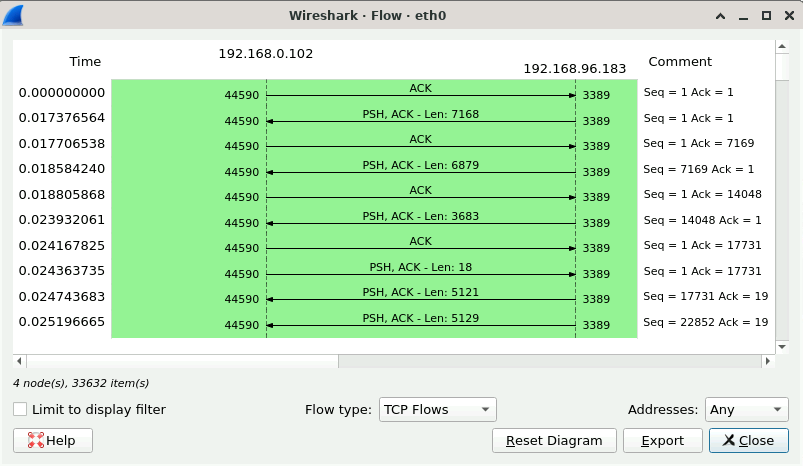
\includegraphics[width=0.8\textwidth]{img/level2/level2-server-flow-analysis.png}
\caption{Wireshark Flow Analysis}\label{fig:WiresharkFlowAnalysis}
\end{figure}

\section{Performance Analysis}

Finally, we assessed the network performance by measuring key metrics such as throughput, delay, and packet loss. Figure~\ref{fig:level2PerformanceAnalysis} summarises the performance analysis results obtained from \texttt{iperf}. The UDP traffic achieved an average bitrate of 3.81 Gbits/sec, which, as we will observe in future levels, is exceptionally high and will drop when we introduce malicious traffic. This baseline measurement provides a reference point for evaluating the impact of network attacks on the overall performance.

\begin{figure}[H]
\centering
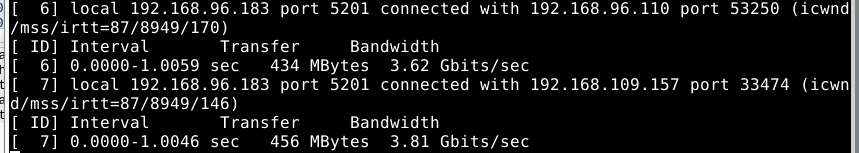
\includegraphics[width=0.8\textwidth]{img/level2/level2-server-performance-analysis.png}
\caption{Performance Analysis}\label{fig:level2PerformanceAnalysis}
\end{figure}